% Source page: original p. 321 (PDF p. 17)
% Figure number: Figure 6
% Uncertainty notes: none
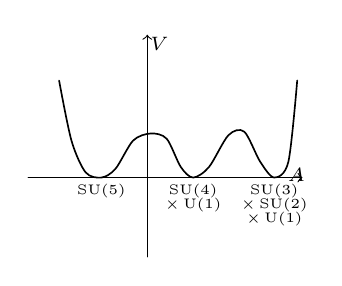
\begin{tikzpicture}[x=1.12cm,y=1.12cm,line cap=round,line join=round]
  \draw[->] (-1.35,0) -- (1.76,0);
  \draw[->] (0,-0.90) -- (0,1.62);
  \node[font=\scriptsize] at (0.14,1.52) {$V$};
  \node[font=\scriptsize] at (1.69,0.03) {$A$};

  \draw[semithick,smooth] plot coordinates {
    (-1.00,1.10) (-0.86,0.42) (-0.70,0.06) (-0.52,0.00)
    (-0.36,0.10) (-0.16,0.42) (0.04,0.50) (0.22,0.44)
    (0.38,0.12) (0.52,0.00) (0.70,0.12) (0.92,0.48)
    (1.10,0.52) (1.28,0.18) (1.44,0.00) (1.60,0.18) (1.70,1.10)
  };

  \node[font=\tiny,anchor=north,inner sep=0pt] at (-0.52,-0.07)
    {$\mathrm{SU}(5)$};
  \node[font=\tiny,align=center,anchor=north,inner sep=0pt] at (0.52,-0.07)
    {$\mathrm{SU}(4)$\\[-1pt]$\times\,\mathrm{U}(1)$};
  \node[font=\tiny,align=center,anchor=north,inner sep=0pt] at (1.44,-0.07)
    {$\mathrm{SU}(3)$\\[-1pt]$\times\,\mathrm{SU}(2)$\\[-1pt]$\times\,\mathrm{U}(1)$};
\end{tikzpicture}
